\chapter{Problemstellung} \label{ch:problem}
In diesem Kapitel wird die Referenzanwendung für diese Arbeit vorgestellt. Zuerst wird auf das benötigte Backend , dessen \textit{\acf{api}} mit Hilfe von \acf{gemara} generiert wurde eingegangen. 
Nach der Vorstellung des \textit{Enfield-Meta-Modell} wird das erzeugte \textit{\acf{api}} dargestellt. Anschließend wird die Android Applikation vorgestellt, wobei in diesem Bereich primär auf das \textit{\acf{ui}} eingegangen wird. Abschließend wird das \textit{Meta-Modell} und mögliche Erweiterungen erläutert und gegeneinander abgewogen.

Um einen Generator zu entwickeln, ist es hilfreich, eine Implementierung der gewünschten Applikation mit all ihren Funktionen und Anforderungen zu erstellen. Bei einer anschließenden Quellcode-Analyse sollte darauf geachtet werden, dass die einzelnen Klassen weitestgehend abstrahiert sind und eine Einteilung in generischen und spezifischen Quellcode erfolgen kann. Der generische Quellcode ist einfacher zu generieren, da dieser statisch ist und sich für alle folgenden Implementierungen nicht verändert. 

\section{Vorstellung der Referenzanwendung}
Die Beispielanwendung soll dem Nutzer die Möglichkeit geben, die Dozenten der Fakultät Informatik der FHWS und deren Ämter einzusehen, einen neuen Dozenten beziehungsweise ein neues Amt anzulegen und zu bearbeiten oder zu löschen. Für jede dieser Aktionen werden entsprechende Endpunkte in dem \textit{\acf{api}} benötigt. Jeder dieser Endpunkte einen Zugriff auf die darunter liegende Datenbank besitzen. Um das zu realisieren, wird ein \textit{Backend-Projekt} mit Hilfe von \ac{gemara} erzeugt.

\newpage

\subsection{Backend Referenzimplementierung}
Dieses Kapitel stellt die Referenzimplementierung des Backends für die Referenzanwendung sowie das \textit{Enfield-Meta-Modell} und das daraus resultierende \textit{\acf{api}} vor.


\subsubsection{\textit{Enfield-Meta-Modell} der Referenzimplementierung} \label{sec:enfield_intro}
Dieses Kapitel befasst sich mit dem benötigten \textit{Enfield-Meta-Modell}. Dafür werden Quellcode-Beispiele aufgezeigt und auf deren Besonderheiten eingegangen. In diesem Kapitel wird nicht das ganze Modell erläutert, sondern nur die wichtigsten Aspekte daraus. Das komplette Modell kann im Anhang unter Listing \ref{lst:enfield_model} eingesehen werden.

In Listing \ref{lst:constructor_enfield} wird die Initialisierung des \textit{Enfield-Modells} dargestellt und die Attribute \textit{producerName}, \textit{packagePrefix} sowie der Name des Projektes festgelegt.

\begin{lstlisting}[label=lst:constructor_enfield,
language=java,
firstnumber=1,
caption=Initialisierung des \textit{Enfield-Meta-Modells}.]	
public MyEnfieldModel() {
	this.metaModel = new Model();

	this.metaModel.setProducerName("fhws");
	this.metaModel.setPackagePrefix("de.fhws.applab.gemara");
	this.metaModel.setProjectName("Lecturer");
}
\end{lstlisting}

Listing \ref{lst:lecturer_res} zeigt, wie eine Ressource angelegt wird, welche einen Dozenten darstellen soll. Der Ressource wird ein Name zugewiesen und sie bekommt einen \textit{MediaType}. Außerdem werden alle Attribute definiert, indem sie benannt und einen Datentyp zugewiesen bekommen.
 Da eines der Attribute eines Dozenten seine Ämter sind, welche als Subressource der \textit{SingleResource Lecturer} dargestellt sind, ist es wichtig, dass das \textit{Enfield-Modell} ebenfalls eine \textit{SingleResource} für diese Ämter besitzt. Dies wird durch den Methodenaufruf \textit{createSingleResourceCharge()} sichergestellt.

\newpage

\begin{lstlisting}[label=lst:lecturer_res,
language=java,
firstnumber=1,
caption=Erzeugung der \textit{SingleResource} \textit{Lecturer}. ]
this.metaModel.addSingleResource("Lecturer");

this.lecturerResource = this.metaModel.getSingleResource("Lecturer");

this.lecturerResource.setModel(this.metaModel);
this.lecturerResource.setResourceName("Lecturer");
this.lecturerResource.setMediaType(
	"application/vnd.fhws-lecturer.default+json");

final SimpleAttribute title = new SimpleAttribute("title", SimpleDatatype.STRING);
[...]
final SimpleAttribute roomNumber = new SimpleAttribute("roomNumber", SimpleDatatype.STRING);
final SimpleAttribute homepage = new SimpleAttribute("homepage", SimpleDatatype.LINK);

createSingleResourceCharge();
final ResourceCollectionAttribute charge = new ResourceCollectionAttribute("chargeUrl", this.chargeResource);

this.lecturerResource.addAttribute(title);
[...]
this.lecturerResource.addAttribute(charge);

addImageAttributeForLecturerResource();
\end{lstlisting}

Sind alle benötigten Ressourcen im Modell definiert, wird der \textit{endliche Automat}, angefangen mit dem \textit{DispatcherState} (Listing \ref{lst:dispatcher_impl}) beschrieben. Dieser bekommt einen Namen, und wird als \textit{DispatcherState} dem Modell hinzugefügt.

\begin{lstlisting}[label=lst:dispatcher_impl,
language=java,
firstnumber=1,
caption=Erzeugung des \textit{DispatcherStates}. ]
final GetDispatcherState dispatcherState = new GetDispatcherState();
dispatcherState.setName("Dispatcher");
dispatcherState.setModel(this.metaModel);
this.metaModel.setDispatcherState(dispatcherState);
this.dispatcherState = dispatcherState;
\end{lstlisting}

\newpage

Beispielhaft für alle nachfolgenden \textit{States} zeigt Listing \ref{lst:getState_impl}, wie der \textit{State GetAllLecturers} erzeugt wird.
Auch dieser \textit{State} bekommt einen Namen. Daneben wird ihm die Ressource zugewiesen, welche er bedienen soll. Neben diesen Eigenschaften werden dem \textit{State} alle \textit{Transitionen} hinzugefügt. In diesem Fall wird zusätzlich dem \textit{DispatcherState} die Information übergeben, dass der \textit{GetAllLecturers State} sein \textit{Folgestate} ist. Alle weiteren \textit{States} werden analog definiert (siehe Listing \ref{lst:enfield_model}).

\begin{lstlisting}[label=lst:getState_impl,
language=java,
firstnumber=1,
caption=Erzeugung des \textit{GetAllLecturers States}. ]
final GetPrimaryCollectionResourceByQueryState getAllLecturersCollectionState = new GetPrimaryCollectionResourceByQueryState();
getAllLecturersCollectionState.setName("GetAllLecturers");
getAllLecturersCollectionState.setModel(this.metaModel);
getAllLecturersCollectionState.setResourceType(this.lecturerResource);

this.dispatcherState.addTransition(new ActionTransition(getAllLecturersCollectionState, "getAllLecturers"));
getAllLecturersCollectionState.addTransition(this.getLecturerByIdState);

this.metaModel.addState(getAllLecturersCollectionState.getName(), getAllLecturersCollectionState);

this.getCollectionOfLecturersState = getAllLecturersCollectionState;
\end{lstlisting}
 
 \newpage
 
\subsubsection{Vorstellung des \textit{\acf{api}}}
Mit Hilfe des zuvor beschriebenen \textit{Enfield-Meta-Modells} wird ein \textit{\acl{api}} generiert, welches in diesem Kapitel vorgestellt wird.
Die Abbildung \ref{fig:api} zeigt das \textit{\acl{api}}, welches für die Beispielanwendung benötigt wird. Dieses\textit{ \ac{api}} entspricht einem \textit{endlichen Automaten} und spiegelt alle Funktionen der Applikation wieder.  

\begin{figure}[H]
	\begin{center}
		\includegraphics[width=\textwidth]{images/api.png}
		\caption{Darstellung des \textit{\ac{api}} der Beispielanwendung.}
		\label{fig:api}
	\end{center}
\end{figure}

\subsection{Android Referenzimplementierung}\label{sec:ref_impl}
Nach der Vorstellung des Backends geht dieses Kapitel darauf ein, wie Informationen des \textit{\acl{api}s} in die Android Applikation einfließen.
Für die Realisierung der gewünschten Funktion werden folgende \textit{Views} benögt: eine \textit{RecyclerView}, welche alle Dozenten in jeweils einer eigenen \textit{CardView} darstellen, eine \textit{DetailView}, welche einen einzelnen Dozenten und all seine Informationen zeigt, jeweils eine \textit{InputView} zur Erzeugung eines neuen Dozenten beziehungsweise zum Bearbeiten eines existierenden Dozenten, eine \textit{RecyclerView}, welche die Ämter eines Dozenten, die Detail-Ansicht eines Amtes anzeigt, sowie jeweils eine \textit{View} zur Bearbeitung beziehungsweise zur Neuanlage eines Amtes.

\subsubsection{\textit{\acf{ui}} der Referenzimplementierung}
In diesem Kapitel wird das \textit{\acl{ui}} der Android Applikation vorgestellt. Dabei wird gezeigt, wie die einzelnen \textit{Views} umgesetzt werden.
Wie dem \acl{api} entnommen werden kann, steigt der Nutzer mit der Liste aller Dozenten in die Applikation ein. Diese Liste ist in diesem Fall, wie in der Einleitung beschrieben, mit einer \textit{RecyclerView} und einzlenen \textit{CardViews} realisiert. Diese Liste kann in Abbildung \ref{fig:list} eingesehen werden.

\begin{figure}[H]
	\begin{center}
		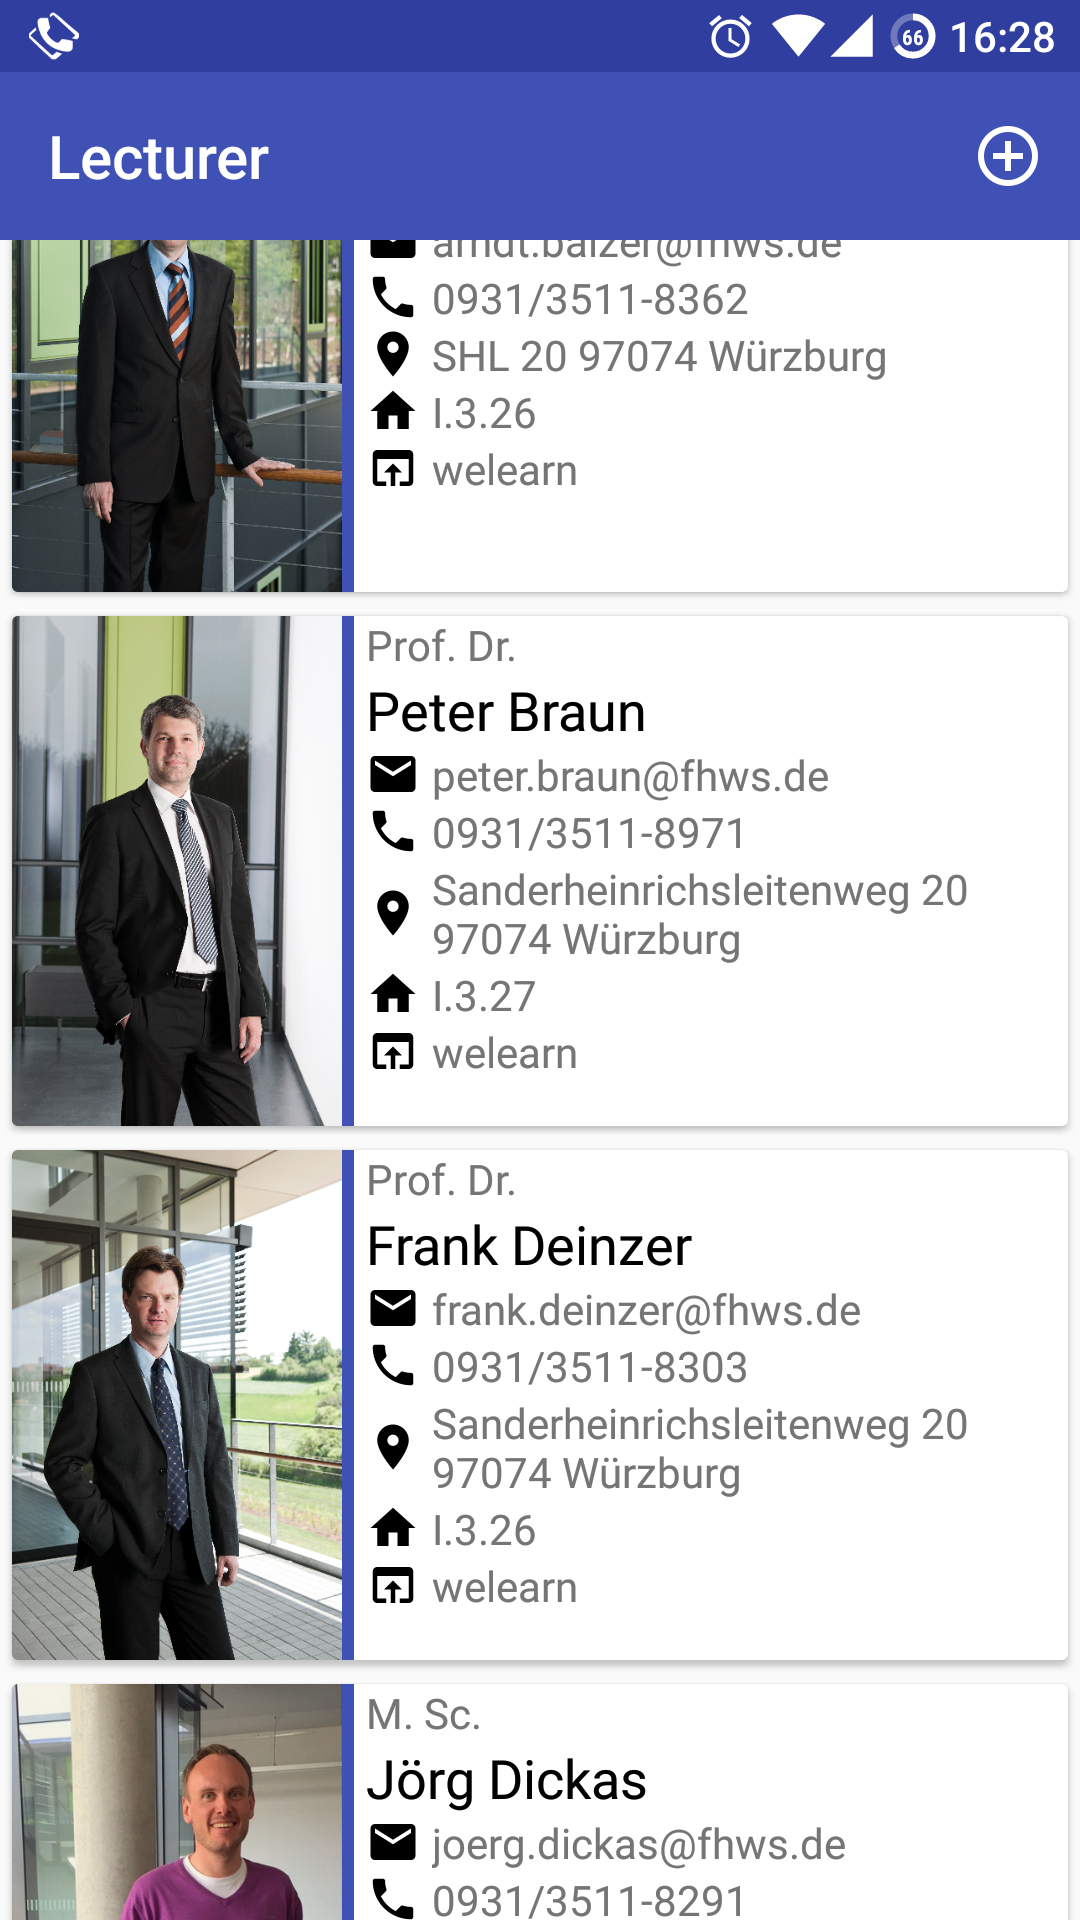
\includegraphics[width=0.4\textwidth]{images/list.png}
		\caption{\textit{RecyclerView} zur Darstellung aller Dozenten.}
		\label{fig:list}
	\end{center}
\end{figure}

Über den \textit{Plus-Button} links oben in der \textit{View} kommt der Nutzer zu der \textit{View}, welche es ermöglicht, einen neuen Dozenten anzulegen. Diese \textit{View} besteht aus \textit{EditText}-Feldern, welche die zur Neuanlage benötigten Informationen vorgeben. Die Abbildung \ref{fig:input_view} zeigt diese \textit{View}. Sie validiert auch, ob eine Eingabe getätigt wurde. Andernfalls wird eine Fehlermeldung angezeigt. Diese Darstellung der Fehlermeldung ist in Abbildung \ref{fig:input_error} dargestellt.

\begin{figure}[H]
	\begin{center}
		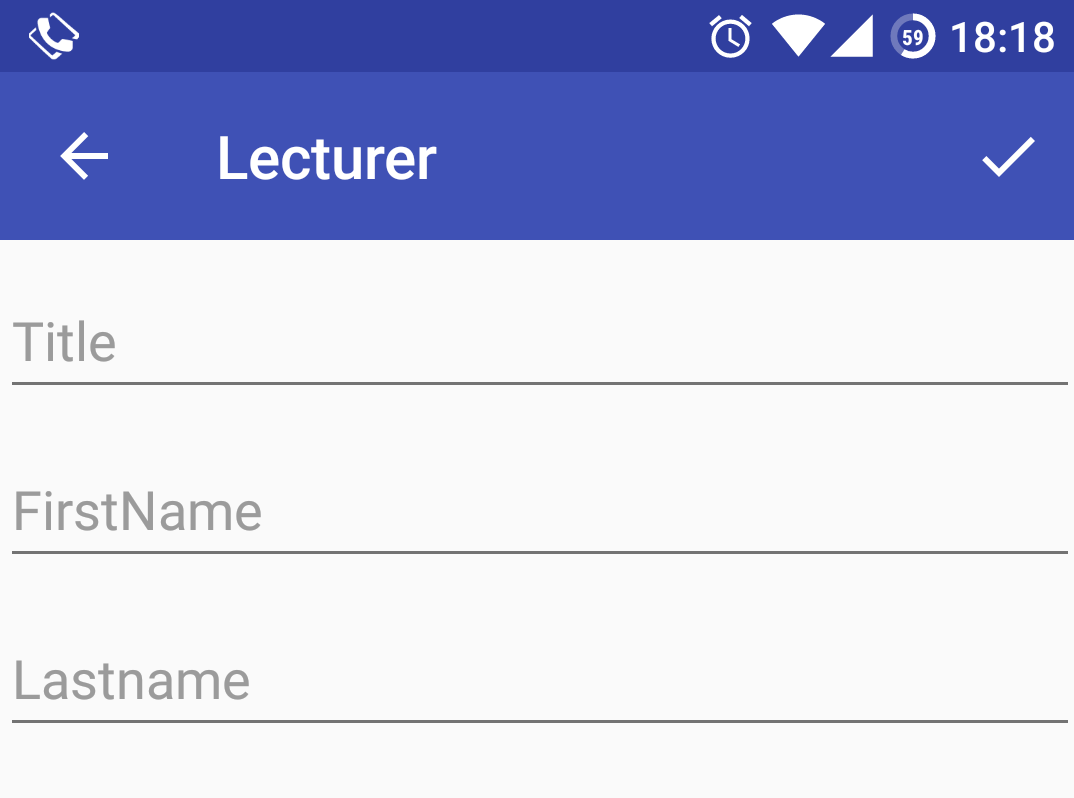
\includegraphics[width=0.4\textwidth]{images/input_small.png}
		\caption{Ausschnitt der \textit{View} zur Erstellung eines Dozenten.}
		\label{fig:input_view}
	\end{center}
\end{figure}

\begin{figure}[H]
	\begin{center}
		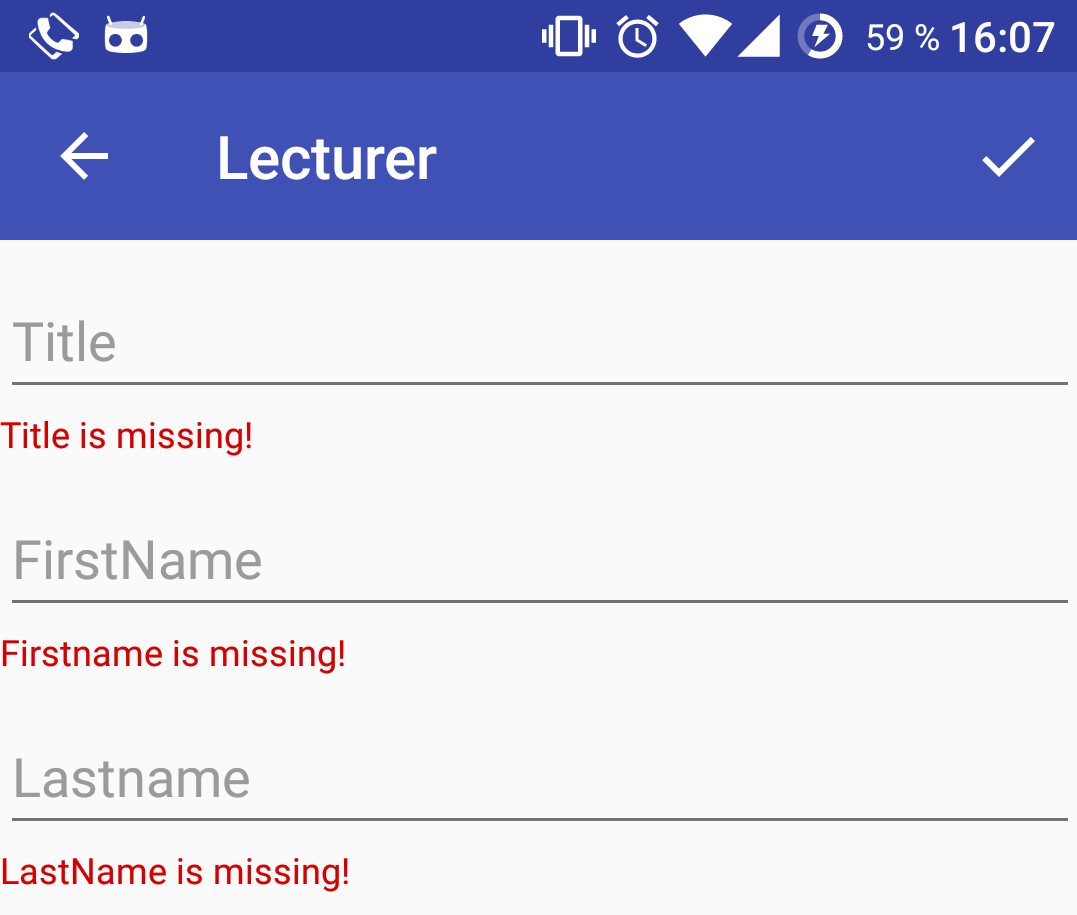
\includegraphics[width=0.4\textwidth]{images/input_error.png}
		\caption{Fehlermeldung bei der Neuanlage eines Dozenten.}
		\label{fig:input_error}
	\end{center}
\end{figure}

Durch die Neuanlage eines Dozenten oder durch den Klick auf seine Karte in der Liste wird der Nutzer auf die Detailansicht eines Dozenten weitergeleitet (Abbildung \ref{fig:detail_view}). Hier besitzt der Nutzer die Option detaillierte Informationen zum betroffenen Dozenten einzusehen. Des Weiteren bekommt er die Möglichkeit, den aktuellen Dozenten zu bearbeiten oder diesen zu löschen. Diese Aktionen können über das Kontextmenü aufgerufen werden. Wobei die \textit{View} zum Editieren des Dozenten analog der \textit{View} zur Neuanlage aussieht mit der Ausnahme, dass die vorhandenen Daten bereits vorausgefüllt sind. Das Löschen des Dozenten wird über einen \textit{Dialog} realisiert. Dieser \textit{Dialog} ist in Abbildung \ref{fig:dialog} dargestellt.

\begin{figure}[H]
	\begin{center}
		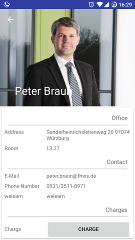
\includegraphics[width=0.4\textwidth]{images/detail.png}
		\caption{Detailansicht eines Dozenten.}
		\label{fig:detail_view}
	\end{center}
\end{figure}

\begin{figure}[H]
	\begin{center}
		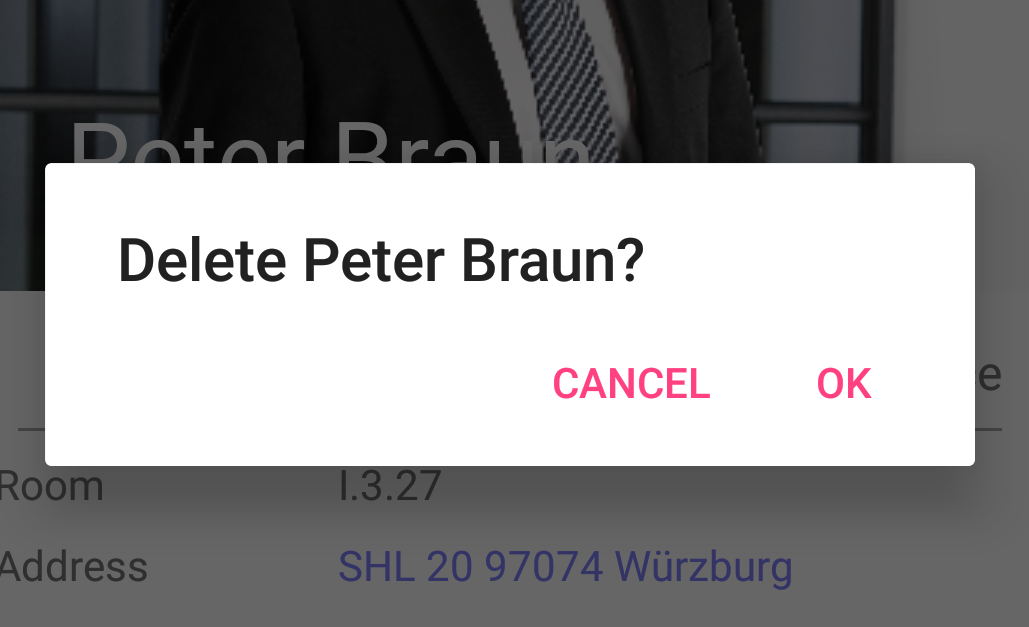
\includegraphics[width=0.4\textwidth]{images/dialog.png}
		\caption{\textit{Dialog} zum Löschen eines Dozenten.}
		\label{fig:dialog}
	\end{center}
\end{figure}

Über den \textit{Charge-Button} gelangt der Nutzer zur Liste mit den Ämtern des Dozenten. Die \textit{Views} für diese Ämter sind analog zu denen der Dozenten. Mit der Ausnahme, dass bei Neuanlage, beziehungsweise beim Bearbeiten eines Amtes dieses mal nicht ausschließlich \textit{EditText} zur Verfügung steht. Da die Ämter die zwei Datumsattribute für den Start und das Ende besitzen, wurde hierfür das \textit{DateTimePicker-Widget} eingebaut. Dieses kann in Abbildung \ref{fig:date} eingesehen werden.

\begin{figure}[H]
	\begin{center}
		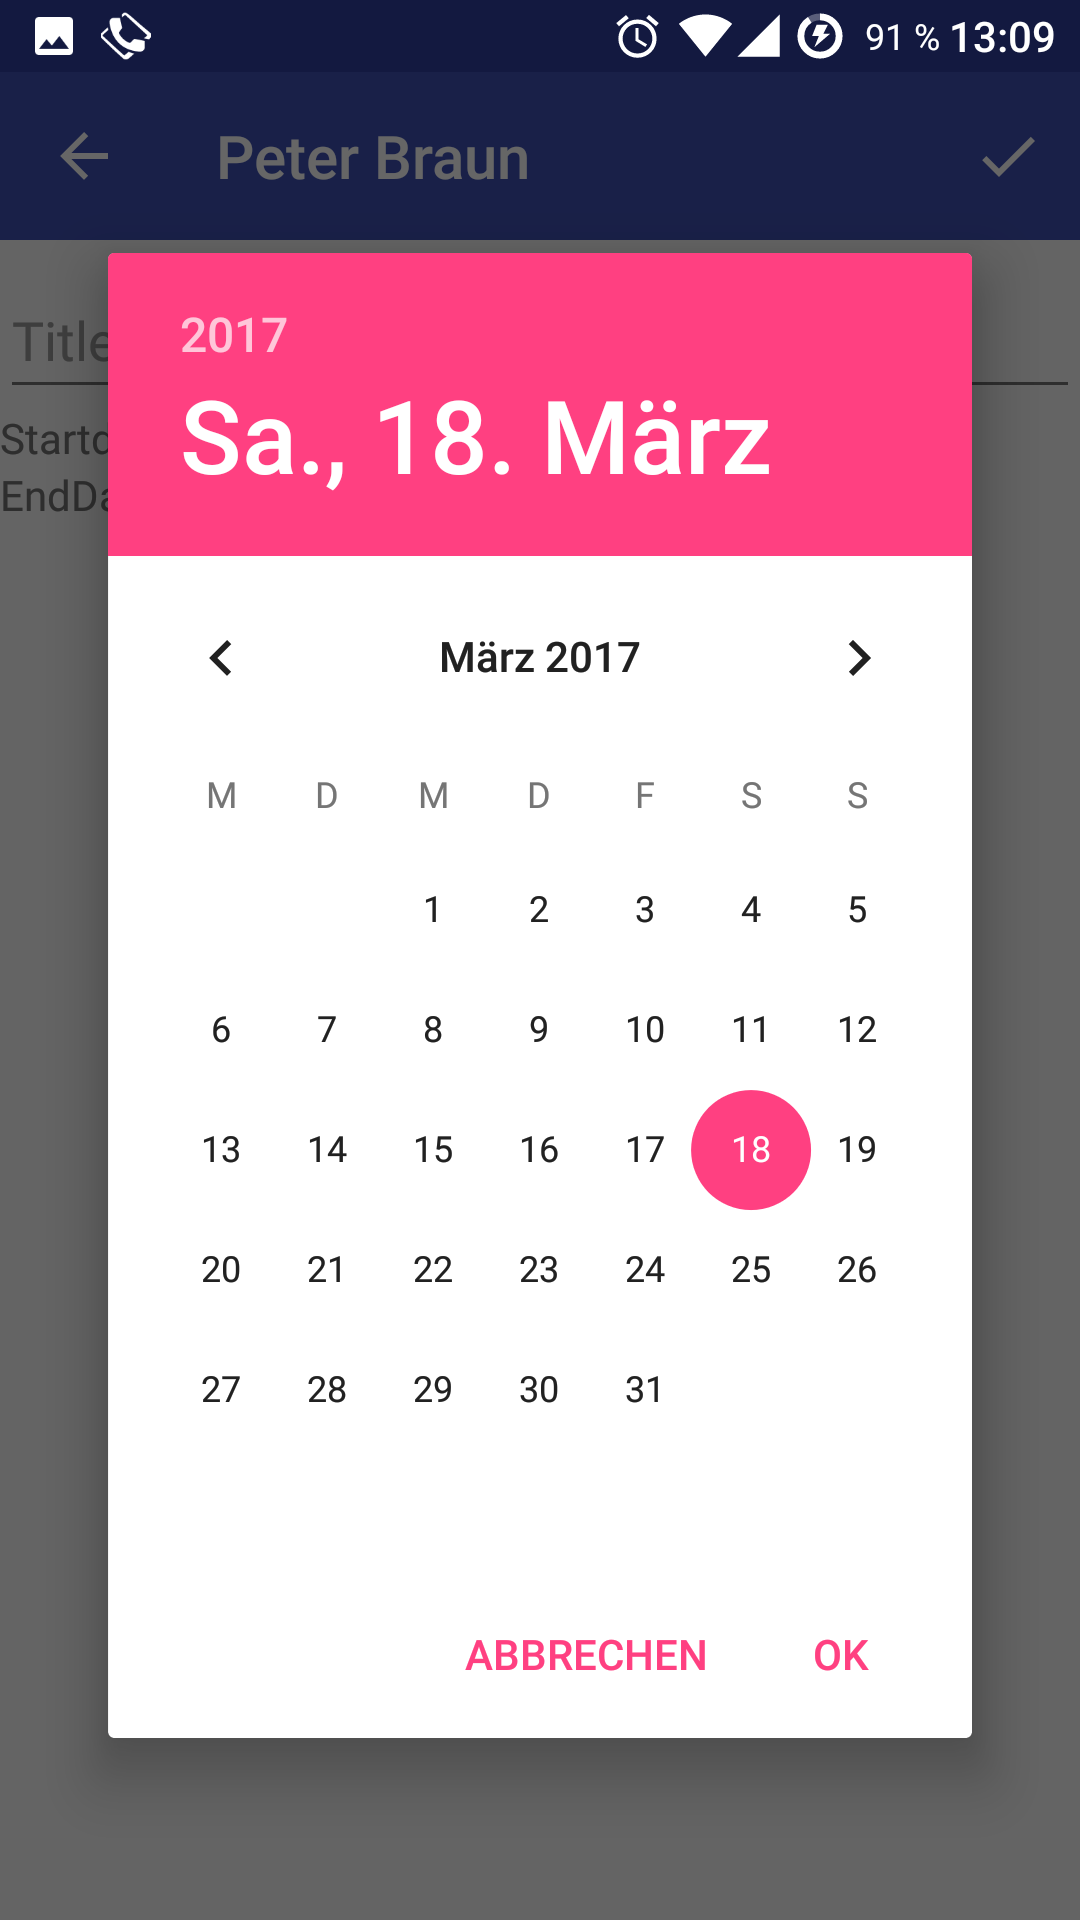
\includegraphics[width=0.4\textwidth]{images/date.png}
		\caption{\textit{DateTimePicker-Widget} zur Datumsauswahl.}
		\label{fig:date}
	\end{center}
\end{figure}

\subsubsection{Zahlen und Fakten}
In diesem Abschnitt sollen Statistiken der Referenzimplementierung vorgestellt werden. So lässt sich die Applikation in zwei Bereiche einteilen: die Applikation an sich, welche den kompletten spezifischen Code und eine Bibliothek besitzt. Diese beinhaltet den kompletten generischen Code sowie die \textit{CustomViews}. Die gesamte Anwendung umfasst ungefähr 3000 \textit{Lines of Java Code} und circa 1000 Zeilen an \textit{XML} Code. 

Die Applikation ist der kleinere Teil der Implementierung. Sie enthält elf Java Klassen, wobei es sich dabei um vier \textit{Activities} und sieben \textit{Fragments} handelt. Daneben besitzt sie sechs Layout-\textit{XML}-Dateien und zwei Animations-\textit{XML}-Dateien. Sowie die üblichen \textit{XML}- und \textit{Gradle}-Dateien.

Die Bibliothek ist mit 44 Java Klassen wesentlich größer als die Applikation, wobei hiervon 15 Klassen spezifischen Code enthalten. Die Klassen lassen sich in \textit{abstrakte Activities}, \textit{abstrakte Fragments}, \textit{abstrakte Adapter}, \textit{abstrakte CustomViews}, \textit{abstrakte Models}, \textit{abstrakte Viewholder},  Klassen für die Netzwerkkommunikation, \textit{Adapter}, \textit{CustomViews}, \textit{Models} und \textit{Viewholder} einteilen. Neben den Java Klassen besteht die Bibliothek aus 14 Layout- und drei Menü-Klassen. Diese 17 Klassen sind alles \textit{XML}-Dateien. Auch die Bibliothek beinhaltet die üblichen \textit{XML}- und \textit{Gradle}-Dateien.

\section{Analyse der Android Anwendung}
Dieses Kapitel beschäftigt sich mit der Android Referenzimplementierung. Es wird der Aufbau der Applikation vorgestellt und anhand dessen analysiert, welcher Programmcode als \textit{Plattformcode} und welcher Programmcode generiert werden muss. Anschließend werden die einzelnen \textit{Views} analysiert. Diese Analyse beschäftigt sich mit dem Design und den Funktionen der \textit{Views}.

\subsection{Analyse des Aufbaus der Android Appliaktion}
Wird der Aufbau der Referenzimplementierung analysiert, so fällt auf, dass es möglich ist, die meisten Klassen soweit zu abstrahieren, dass diese keine projekt-spezifischen Informationen mehr enthalten, im Falle dieser Referenzimplementierung keine Informationen zu Dozenten oder deren Ämter. Die Klassen ohne diese spezifischen Informationen werden im Folgenden als \textit{Plattformcode} oder generischer Code bezeichnet. Das Ziel bei der Referenzimplementierung ist, möglichst viel \textit{Plattformcode} und möglichst wenig spezifischen Code in der Anwendung zu haben. 

Das Schaubild \ref{fig:lecturer_structure} verdeutlicht das Verhältnis von generischen (weiße Kästen) und spezifischen (rote Kästen) Klassen. Die Anzahl der gleichbleibenden Klassen ist mit etwa 60 Prozent bereits höher als der Anteil an spezifischen Klassen. Je höher der Anteil dieser unveränderlichen Klassen, desto geringer wird die Komplexität des Generators. Da der Aufwand, eine spezifische Klasse zu erzeugen, mehr Logik benötigt, als eine Klasse, welche immer gleich bleibt.

\begin{figure}[H]
	\begin{center}
		\includegraphics[width=\textwidth]{images/Lecturer.png}
		\caption{Aufbau der Referenzimplementierung.}
		\label{fig:lecturer_structure}
	\end{center}
\end{figure}

Daneben zeigt die Abbildung \ref{fig:lecturer_structure} auch noch die Aufteilung der Klassen in Klassen der Applikation (gestrichelte Kästen) und Klassen der Bibliothek (solide Kästen). Die Applikation an sich besteht nur aus ein paar wenigen \textit{Fragmenten} und \textit{Activities}, welche alle projektspezifisch sind. Der komplette generische Quellcode befindet sich in der Bibliothek. Des Weiteren befinden sich dort auch die spezifischen Komponenten, beispielsweise der \textit{LecturerInputView}. Diese Komponente kann in den Fragmenten zur Bearbeitung oder Neuanlage eines Dozenten mit wenigen Zeilen Programmcode verwendet werden.

Diese Art der Aufteilung ermöglicht, dass ein Applikations Entwickler sich die Komponente, für das Anzeigen, Bearbeiten, Löschen und der Neuanlage generieren lassen, diese Komponenten jedoch beliebig in seiner eigenen Applikation verwenden kann.


\subsection{Analyse der Android \textit{Views}}
In diesem Kapitel sollen die \textit{Views} der Android Applikation an sich analysiert werden. Hierfür werden die Bereiche Aufbau der \textit{Views}, Darstellung von Schrift und Aktionen bei Klick genauer betrachtet. Um ein \textit{Meta-Modell} für Android Anwendungen zu entwickeln, muss der Designer untersuchen, welche Eigenschaften dieses Modell besitzen soll. Diese Eigenschaften spiegeln die Möglichkeiten wider, die Android Anwendung zu beschreiben. Für das Extrahieren dieser Eigenschaften ist ein guter Ansatz, eine Referenzimplementierung, zu entwickeln. Diese Referenz dient fortan als Beispiel. Weiterhin stellt sie das erste zu erreichende Ziel dar. Alle Bemühungen müssen darauf hinauslaufen, eine Applikation generieren zu lassen, welche der Referenzimplementierung gleicht.

Schon beim Entwickeln der Referenz muss sich der Entwickler Gedanken darüber machen, welche \textit{Views} die Anwendung besitzen soll. Diese \textit{Views} entscheiden auch über die Funktionalitäten, welche der Entwickler den Nutzern zur Verfügung stellen will. So wird bereits bei der Planung und Entwicklung der Applikation festgehalten, welche Features realisiert werden. Dieser Funktionsumfang beschreibt, ob der Nutzer Listen- und Detailansichten zur Verfügung hat und ob er Datensätze löschen, neu anlegen beziehungsweise bearbeiten darf. Mit der Entscheidung, dass es eine Möglichkeit zur Neuanlage und Bearbeitung von Datensätzen geben soll, muss zusätzlich festgelegt werden, welche Attribute des Datensatzes bearbeitet werden dürfen und welche minimal notwendig sind.

Ist bekannt, welche \textit{Views} realisiert werden, muss über den Aufbau der einzelnen \textit{Views} entschieden werden. Es müssen Entscheidungen über die Anordnung der darzustellenden Informationen innerhalb einer \textit{View} getroffen werden. Diese Entscheidungen beinhalten neben der Strukturierung und Darstellung textueller Informationen auch Überlegungen zum Erscheinungsbild. Dazu gehören Eigenschaften wie Schriftgröße oder Schriftfarbe. Ist eine \textit{View} fertig designed, steht fest, in welcher Reihenfolge gegebene Informationen angezeigt werden und ob Informationen wie Vorname und Nachname zusammengefasst werden.
Der Entwickler muss entscheiden ob alle bereitgestellten Informationen in der entsprechenden Ansicht relevant sind oder ob auf einzelne Daten verzichtet werden kann. Existieren unter den Daten Bilder, so muss klar sein wo diese platziert werden sollen.

Neben diesen auf das \textit{\acf{ui}} bezogenen Kriterien müssen Entscheidungen darüber gefällt werden, ob die angezeigten Informationen ausschließlich informative Details oder ob diese interaktiv sind. Das heißt, der Benutzer der Android Applikation soll die Möglichkeit haben, weitere Funktionen durch das Anklicken einer dieser Felder auszuführen. Mögliche Aktionen wären beispielsweise das Öffnen der Anwendung \textit{Maps} beim Klick auf eine Adresse oder das Öffnen eines Webbrowsers beim Anklicken eines Hyperlinks. 

All diese Entscheidungen, welche über den Aufbau und das Design der Android Applikation entscheiden, sind für einen Generator wichtig. Dieser benötigt alle Informationen, um sie in der zu generierende Anwendung zu realisieren. Hierfür muss ein \textit{Meta-Modell} entwickelt werden, welches alle oben genannten Beschreibungen im Bezug zur Android Applikation widerspiegelt. Das Modell muss alle Informationen über die Anzahl und Arten der \textit{Views}, deren Aufbau und die exakte Darstellung von Schrift, Bildern und möglichen Funktionen, welche bei Klick ausgeführt werden sollen, besitzen.

\section{\textit{Meta-Modell}}
Nach der Vorstellung und Analyse der Referenzimplementierung, wurden alle relevanten Informationen erkannt und zusammengestellt. Diese Zusammenstellung an Daten, welche die Applikation beschreiben, wird \textit{Meta-Modell} genannt.

\subsection{Kompatibilität mit \acs{gemara} und anderen möglichen Clients}
Da Enfield primär für die Generierung von Anwendungen im \textit{Backend}-Bereich entwickelt wurde, in welchem die Gestaltung von \textit{User Interfaces (UI)} eine eher untergeordnete Rolle spielen, muss die Erweiterung auch dieses Feature realisieren. Neben all der Erweiterungen muss sichergestellt werden, dass das \textit{Meta-Modell} auch weiterhin für das Generieren von \textit{Backends} genutzt werden kann. Idealerweise, ohne die Überarbeitung der bereits entwickelten Software-Generatoren. 

Die Abbildung \ref{fig:enfield-model} zeigt die vereinfachte Modell-Klasse des \textit{Enfield-Meta-Modells}. 
In dieser Klasse sind bereits die wichtigsten Informationen, wie zum Beispiel der Name der Applikation oder unter welchem \textit{Package} diese zu finden ist, vorhanden. Neben diesen grundsätzlichen Informationen liefert die Modell-Klasse auch den Startpunkt des \textit{endlichen Automaten}, welcher die Anwendung definiert. Dieser Startpunkt ist der \textit{GetDispatcherState}. Dieses Objekt besitzt das Attribut \textit{transitions}. Dieses Attribut gibt an, welche \textit{States} auf den \textit{Dispatcher-State folgen}. Jeder dieser folgenden \textit{States} besitzt wiederum eine Collection mit \textit{Transitionen}, welche auf die nachfolgenden \textit{States} verweisen. So wird mit Hilfe der \textit{Transitionen} und der \textit{States} der \textit{endliche Automat} beschrieben. Der Generator kann diese Beschreibung nutzen, um zu entscheiden, in welcher Reihenfolge welche Klassen generiert werden müssen.

\begin{figure}[H]
	\begin{center}
		\includegraphics[width=0.86\textwidth]{images/Enfield-Meta-Model.png}
		\caption{Vereinfachter Aufbau des \textit{Enfield-Meta-Modells}.}
		\label{fig:enfield-model}
	\end{center}
\end{figure}

Um die zusätzlich benötigten Informationen für die Android Applikation in dieses bestehende Modell einzubauen, gibt es zwei Optionen:

\subsection{Definition eines eigenen \textit{Android-Meta-Modells}}

Es besteht die Möglichkeit, die Modell-Klasse um ein Attribut \textit{Android-Meta-Modell} zu erweitern.
Die Abbildung \ref{fig:android-model} zeigt schemenhaft ein Beispiel, wie ein \textit{Android-Meta-Modell} aussehen könnte. Auffällig hierbei ist, dass viele Informationen, die das \textit{Enfield-Modell} bereits liefern würde, noch einmal explizit beschrieben werden. Ein Beispiel sind die \textit{Transitionen} zwischen den \textit{Fragmenten}, beziehungsweise zwischen den \textit{Activities}. 


Der Nutzer des Software-Generators muss ziemlich viel über den Ablauf und die Funktionsweise einer Android-Anwendung wissen, um diesen Generator sinnvoll verwenden zu können.
Dabei bleibt zusätzlich noch die Möglichkeit, dass der Nutzer eigens geschriebene Methoden in das Modell einpflegen kann. John Abou-Jaoudeh et al. haben in ihrer Arbeit ein \textit{Meta-Modell} entwickelt, welches genau solche Features unterstützt\cite{abou2015high}.

\newpage

Der Vorteil einer solchen Erweiterung des \textit{Enfield-Modell}s ist, dass alle benötigten Daten für die Android Anwendung an einer Stelle zu finden sind. Auch hat der Nutzer die Möglichkeit an manchen Stellen eigene Methoden einzufügen weshalb er in der Lage ist das Verhalten der Applikation weiter zu individualisieren.

Jedoch überwiegen in diesem Fall die Nachteile. Ein Nachteil dieses Vorgehens ist die redundante Beschreibung des Programm-Ablaufes. Einmal im \textit{Android-Meta-Modell} und einmal im \textit{Enfield-Meta-Modell}. Bei jeder Änderung gilt dies zu berücksichtigen. 
Weitergehend negativ zu bewerten ist, dass der Nutzer des Software-Generators sich in der Entwicklung von Android Anwendungen auskennen muss. Er muss genau das Zusammenspiel von \textit{ViewHoldern}, \textit{Adaptern}, \textit{Fragments} und \textit{Activities} kennen. Er muss wissen, wie diese ineinandergreifen und wann welche Aktionen ausgelöst werden müssen. Weiterhin sollte er ein grundsätzliches Verständnis für das \textit{\acf{mvc} Pattern} besitzen, welches bei der Entwicklung von Android Applikationen Anwendung findet.
Ein weiterer Nachteil ist die Beschränkung des Modells auf Android. Wird das \textit{Enfield-Modell} um ein \textit{Android-Meta-Modell} erweitert, so muss dies für jeden einzelnen \textit{Client} geschehen. Soll der Generator beispielsweise um Polymer-Webkomponenten oder eine iOS-Anwendung erweitert werden, so müsste für jede einzelne Art von \textit{Client} das \textit{Enfield-Modell} mit einem entsprechenden \textit{Meta-Modell} angepasst werden.

\begin{figure}[H]
	\begin{center}
		\includegraphics[width=0.86\textwidth]{images/Android-Meta-Model.png}
		\caption{Möglicher Aufbau eines \textit{Android-Meta-Modells}.}
		\label{fig:android-model}
	\end{center}
\end{figure}

\subsection{Allgemeine Erweiterungen des \textit{Enfield-Modells}}\label{sec:generic_modell}

In dieser Arbeit wurde sich für die Variante entschieden, das \textit{Enfield-Modell} an geeigneter Stelle zu erweitern.
Diese Stelle befindet sich in den einzelnen \textit{States}. Jede Instanz des \textit{AbstractState} besitzt ein Attribut \textit{SingleResourceView}. Diese Klasse wird um die  Attribute, welche benötigt werden, ergänzt. In der Abbildung \ref{fig:enfield-model-extended} ist der vereinfachte Aufbau des \textit{AbstractStates} und einer \textit{SingleResourceView} zu sehen.

\newpage

Wird beispielsweise eine Instanz eines \textit{GetPrimarySingleResourceByIdStates} erzeugt, und dessen \textit{SingleResourceView} enthält alle notwendigen Informationen, um die \textit{View} in der Android Anwendung zu beschreiben, kann der Generator mit Hilfe der \textit{Transitionen} über die \textit{States} iterieren und verfügt an jedem \textit{State} über alle benötigten Informationen, um den aktuellen \textit{State} in der Anwendung generieren zu lassen.

Bei dieser Methode befinden sich alle \textit{state}-spezifischen Daten direkt am \textit{State}. Jedoch gibt es neben diesen spezifischen Daten auch Daten, welche die komplette Applikation betreffen. Hierfür muss das \textit{Enfield-Modell} noch an einer anderen Stelle erweitert werden. 
Es erscheint sinnvoll, die Erweiterung direkt in der Modell-Klasse vorzunehmen. So kann der Generator schon am Anfang auf diese Daten zugreifen und diese verarbeiten.

Die Abbildung \ref{fig:enfield-model-extended} zeigt das \textit{Enfield-Modell}, welches um die oben genannten Informationen erweitert wurde.

\begin{figure}[H]
	\begin{center}
		\includegraphics[width=0.86\textwidth]{images/Enfield-Meta-Model-Erweitert.png}
		\caption{Vereinfachter Aufbau des erweiterten \textit{Enfield-Meta-Modells}.}
		\label{fig:enfield-model-extended}
	\end{center}
\end{figure}

Der Nachteil dieser Methode ist, das die Informationen an mehr als einer Stelle im \textit{Enfield-Modell} zu finden sind. Sollten die Informationen zu den \textit{Clients} verändert werden, so sind Änderungen an der \textit{SingleResourceView}-Klasse und in der Modell-Klasse nötig. Die Vorteile wurden jedoch zuvor, in Abschnitt \ref{sec:generic_modell}, schon einmal erwähnt. Der Generator kann das Modell als Fahrplan nutzen und weiß genau, wann er welche Klassen für die Android Anwendung erzeugen muss. Er kann auch mit Hilfe der \textit{Transitionen} bestimmen, wie der Verlauf innerhalb der Anwendung gestaltet sein soll.

\subsection{Analyse der benötigten Dateien für das \textit{Meta-Modell}}

Nachdem identifiziert wurde, an welchen Stellen das \textit{Enfield-Modell} erweitert werden soll, folgt die Analyse, welche Informationen an diesen Stellen zur Verfügung gestellt werden müssen. Dabei muss auch ein Augenmerk auf die Aufbereitung der Informationen darauf gelegt werden, dass diese nicht nur eine Android-Applikation, sondern auch mögliche andere \textit{Clients} unterstützen.

Die Analyse in dieser Arbeit beschränkt sich auf die \textit{Clients} Android und Polymer-Webkomponente. Bei beiden wird das \acf{ui} nach den Richtlinien des von Google entwickelten Material Design erstellt \cite{material}. Diese Richtlinien schreiben bereits viele nötige Informationen für die Oberflächengestaltung vor. So wird beispielsweise definiert, dass Einträge in einer Liste als Karte dargestellt werden sollen. Abstände und Icons werden ebenfalls festgelegt.

\subsubsection{CardView}

\begin{figure}[H]
	\begin{center}
		
\includegraphics[width=0.75\textwidth]{images/card.png}
		\caption{Beispiel einer \textit{CardView} eines Dozenten nach Material Design.}
		\label{fig:card}
	\end{center}
\end{figure}

\newpage

\begin{lstlisting}[label=lst:braun_json,
language=json,
firstnumber=1,
caption=Demo Daten eines Dozenten.]	
[...]	   
{
"address": "Sanderheinrichsleitenweg 20 97074 Wuerzburg",
"chargeUrl": {
"href": "https://apistaging.fiw.fhws.de/mig/api/lecturers/4/charges",
"rel": "chargeUrl",
"type": "application/vnd.fhws-charge.default+json"
},
"email": "peter.braun@fhws.de",
"firstName": "Peter",
"homepage": {
"href": "http://www.welearn.de/[...]/prof-dr-peter-braun.html",
"rel": "homepage",
"type": "text/html"
},
"id": 4,
"lastName": "Braun",
"phone": "0931/3511-8971",
"profileImageUrl": {
"href":"https://apistaging.fiw.fhws.de/[...]/4/profileimage",
"rel": "profileImageUrl",
"type": "image/png"
},
"roomNumber": "I.3.27",
"self": {
"href": "https://apistaging.fiw.fhws.de/mig/api/lecturers/4",
"rel": "self",
"type": "application/vnd.fhws-lecturer.default+json"
},
"title": "Prof. Dr."
}
[...]
\end{lstlisting}


Die  \textit{\acf{json}} Repräsentation unter Listing \ref{lst:braun_json} beschreibt das Beispiel aus Abbildung \ref{fig:card}.
Jetzt gilt es zu überlegen, wie die Attribute des \textit{JSON} Objekts aufzubereiten sind, dass diese die Karte des Dozenten widerspiegeln. In erster Linie muss entschieden werden, welche der gelieferten Informationen in der Liste für jeden einzelnen Dozenten angezeigt werden sollten. Ist es sinnvoll Informationen zu gruppieren? Hier beispielsweise die Attribute \textit{firstName} und \textit{lastName}, welche in einer Zeile angezeigt werden sollen. Ist bekannt welche Informationen eine Karte enthalten soll, so muss auch die Reihenfolge der einzelnen Attribute auf der Karte bestimmt werden. Neben der Reihenfolge gibt es außerdem die Möglichkeit, Schriftgröße oder Schriftfarbe der einzelnen Attribute unterschiedlich zu gestalten. Auch müssen die Standardicons den jeweiligen Attributen zugewiesen werden. Es sollte zudem möglich sein, einzelnen Attributen bestimmte Aktionen zuzuweisen. Beispielsweise sollte beim Klick auf eine Homepage, diese im Browser geöffnet werden oder beim Klick auf die Adresse sollte sich die Applikation \textit{Maps} öffnen und die angeklickte Adresse dort anzeigen. Bei einem Attribut mit Hyperlink zu einer Website sollte es möglich sein, einen mitgegebenen Text anstelle des Hyperlinks anzuzeigen.
Besitzt die Karte ein Bild, so sollte der Nutzer die Möglichkeit besitzen, zu entscheiden, ob dieses auf der linken oder rechten Seite der Karte dargestellt werden soll.


\subsubsection{\textit{DetailView}}

\begin{figure}[H]
	\begin{center}
		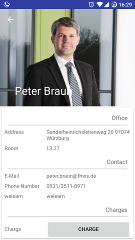
\includegraphics[width=0.4\textwidth]{images/detail.png}
		\caption{Beispiel einer \textit{DetailView} eines Dozenten nach Material Design.}
		\label{fig:detail}
	\end{center}
\end{figure}

Die zur Verfügung stehenden Daten sind die, die unter Listing \ref{lst:braun_json} einzusehen waren.

Analog zu der \textit{CardView} stellt sich auch bei der \textit{DetailView} die Frage, welche Daten dargestellt werden sollen. Hier jedoch gibt es zusätzlich zu der horizontalen Gruppierung (Beispiel: Vornamen und Nachnamen) auch noch eine vertikale Gruppierung. Diese wird im Weiteren auch Kategorisierung genannt. In der detaillierten Ansicht eines Dozenten gibt es die Möglichkeit, Attribute zu kategorisieren und jede Kategorie mit einem Namen zu versehen. Für die Gestaltung und Anordnung sowie mögliche Klick-Aktionen müssen die selben Anforderungen wie bei der \textit{CardView} berücksichtigt werden. 

Jedoch muss die \textit{DetailView} wissen, welches Attribut den Titel der \textit{View} darstellt, da dieser in der \textit{AppBar} erscheinen wird. In diesem Beispiel ist es der Name des Dozenten. Anders als bei der \textit{CardView} gibt es hier nicht die Möglichkeit zu bestimmen, an welcher Stelle das Bild dargestellt werden soll. Ist ein Bild vorhanden, so wird dieses in der \textit{CollapsingToolbar} dargestellt \cite{collapsing}.

\subsubsection{InputView}

\begin{figure}[H]
	\begin{center}
		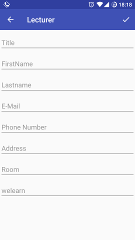
\includegraphics[width=0.4\textwidth]{images/input.png}
		\caption{Beispiel einer \textit{View} zum Anlegen eines Dozenten.}
		\label{fig:input}
	\end{center}
\end{figure}

\newpage

Für das Anlegen eines Dozenten oder auch zum Bearbeiten muss entschieden werden, welche Attribute zum Anlegen nötig sind. Auch hier ist es notwendig, die Reihenfolge zu bestimmen. Jedoch kommt in dieser \textit{InputView} für jedes Attribut noch die Option hinzu, einen \textit{Hint}-Text anzugeben. Dieser Text beschreibt, was innerhalb der Android-\textit{View} \textit{EditText} als Beschreibung für das bestimmte Attribut steht. Weiter sollte es die Möglichkeit geben, jedem Feld eine Nachricht, welche angezeigt wird, wenn das Feld beispielsweise leer gelassen wird oder eine weitere Nachricht mitzugeben, wenn das Eingegebene nicht dem Erwarteten entspricht, zum Beispiel wenn in das Feld für die E-Mail eine Telefonnummer eingegeben. Oder ein regulärer Ausdruck mitgegeben wurde und das Eingegebene nicht dessen Anforderungen entspricht.

\subsubsection{Programmablauf und Klick-Aktionen}

Da das \textit{Enfield-Modell} bereits einen \textit{endlichen Automaten} beschreibt, welcher den Programmablauf widerspiegelt, ist es nicht notwendig, diesen noch einmal genauer zu definieren, sondern es kann der bereits definierte Ablauf übernommen werden.

Auch die Aktionen, welche durch einen Klick auf ein bestimmtes Attribut ausgeführt werden sollen, beschränken sich auf Android Standardaktionen, beispielsweise das Wechseln zu den \textit{Maps}, zu einem \textit{E-Mail Client}, dem \textit{Browser} oder zum \textit{Anrufmenü}. Jede dieser Aktionen ergibt sich aus den Typen der Attribute, weswegen diese auch nicht weiter definiert werden müssen.

\subsection{Design der \textit{View-Meta-Modelle}} \label{sec:resourceViews}

In den letzten Abschnitten der Arbeit wurde aufgezählt, welche Eigenschaften das \textit{Meta-Modell} sowohl android- als auch polymerseitig besitzen muss. In diesem Kapitel wird ein \textit{Meta-Modell} vorgestellt, welches die erwähnten Eigenschaften abdeckt.


\begin{figure}[H]
	\begin{center}
		\includegraphics[width=\textwidth]{images/metamodel.png}
		\caption{Aufbau der \textit{Views} zur Erweiterung des \textit{Enfield-Modell}s.}
		\label{fig:meta-model}
	\end{center}
\end{figure}

Die Abbildung \ref{fig:meta-model} zeigt den Aufbau der Objekte, mit welchem das \textit{Enfield-Modell} erweitert wird. Die drei \textit{Views}: \textit{CardView}, \textit{DetailView} und \textit{InputView} sind alles Instanzen von \textit{AbstraktResourceView}. Jede \textit{View} weiß, durch die Zuordnung mit Hilfe des Ressourcennamens, welche Ressource sie darstellen soll. Die drei \textit{Views} lassen sich in zwei Kategorien einteilen: \textit{Views}, welche Informationen anzeigen und \textit{Views}, welche zur Eingabe von Informationen benötigt werden.
So gehören \textit{CardView} und \textit{DetailView} zu den anzeigenden \textit{Views} und die \textit{InputView} zur zweiten Kategorie. 

\subsubsection{Anzeigende \textit{Views}}
Diese \textit{View}-Typen haben die Aufgabe, eine Liste aller Attribute zu halten, welche in der entsprechenden \textit{View} angezeigt werden sollen. Dabei bestimmt die Reihenfolge, in welcher die Attribute in dieser Liste sind, auch die Anordnung in der Oberfläche. Ist das erste Item in der Liste der Name, so wird dieser ganz oben in der \textit{View} angezeigt.
Bei der \textit{DetailView} jedoch gibt es nicht eine Liste mit Attributen, sondern eine Liste mit Kategorien. Diese besitzen 
einen Namen und eine Liste mit den Attributen ihrer Kategorie. Die Darstellungsreihenfolge der Kategorien und deren Attribute ist analog zu der der \textit{CardView}. Weiter besitzt die \textit{DetailView} das Attribut \textit{image}. Dieses wird hier aus der Liste der Attribute herausgezogen, da dieses Attribut bestimmt, ob die \textit{View} eine \textit{CollapsingToolbar} besitzen wird oder nicht. Wiederum haben beide \textit{Views} das Attribut \textit{titleOfResource}. Dieses bestimmt, welches Attribut unserer Ressource beispielsweise in der \textit{Toolbar} angezeigt wird.

Auf die polymerspezifischen Attribute wird in dieser Arbeit nicht weiter eingegangen.

Mit Hilfe der Listen, den Titelattributen und dem Bildattribut kann das Erscheinungsbild einer \textit{View} gut beschrieben werden. Als nächstes wird auf die Möglichkeiten, Schriftgrößen, Schriftfarben und Klick-Aktionen zu definieren eingegangen.
Außerdem ist es bis jetzt nur möglich, einfache Attribute anzuzeigen. Eine horizontale Gruppierung ist noch nicht umsetzbar. Um diese Anforderungen zu erfüllen, werden nicht Attribute in den Listen gespeichert, sondern Ausprägungen von \textit{ResourceViewAttributen}. 

Es gibt zwei Ausprägungsarten: \textit{SingleResourceViewAttribute} und \textit{GroupedResourceViewAttribute}.  Das \textit{SingleResourceViewAttribute} ist für einfache Attributn. Mit diesen ist es beispielsweise möglich, den Titel eines Dozenten anzuzeigen. Das \textit{GroupedResourceViewAttribute} ermöglicht die horizontale Gruppierung. Beide Objekte bestimmen jedoch nicht die designspezifischen Eigenschaften des Attributs. Hierfür besitzen beide Attributtypen das Attribut \textit{DisplayViewAttribute}.

Während bei der \textit{SingleResourceViewAttribute} das \textit{GroupedResourceViewAttribute} wiederum gibt eine Liste von diesen \textit{DisplayViewAttributen}, welche die anzuzeigenden Informationen widerspiegeln. Weitergehend besitzt das \textit{GroupedResourceViewAttribute} auch ein \textit{DisplayViewAttribute}, welches die neu entstandene Gruppierung beschreiben soll.

Ein \textit{DisplayViewAttribute} ist nun in der Lage, Schriftgröße und -farbe zu definieren. Die angegebene Farbe muss in hexadezimaler Darstellung angegeben werden. Wird keine Farbe mitgegeben, wird die Defaultfarbe der Anwendung genommen. In der Regel ist diese schwarz. Die Schriftgröße wiederum ist auf drei Stufen beschränkt. Es gibt die Möglichkeit, den Text in klein, normal und groß darzustellen. Per Default ist normal eingestellt. Wegen der Oberklasse \textit{AbstractViewAttribute} besitzt das \textit{DisplayViewAttribute} noch das Attribut \textit{attributeName}. Dieses muss exakt so heißen, wie in der Definition der Ressource.
Mit dem \textit{attributeLabel} kann angegeben werden, wie dieses Attribut in der \textit{View} angezeigt werden soll. Die Abbildung \ref{fig:detail} zeigt die Verwendung von den Labels, Beispielsweise steht von der E-Mailadresse des Dozenten \textit{E-Mail}. Dieser String entspricht dem Label des Attributs. Weiterhin muss angeben werden, von welchem Typ das aktuell beschriebene Attribut ist.
Dies geschieht mit dem Attribut, \textit{AttributeType}. Es gibt folgende mögliche Typen: \textit{HOME}, \textit{MAIL}, \textit{LOCATION}, \textit{PICTURE}, \textit{PHONE\_NUMBER}, \textit{TEXT}, \textit{URL}, \textit{DATE}, \textit{SUBRESOURCE}. Jeder Typ bestimmt die Eigenschaften des Attributs. Über diesen wird bestimmt, welches Icon in der Karte vor dem entsprechenden Attribut angezeigt wird oder welche Aktion bei Klick ausgeführt werden soll. So wird bei einem Klick auf ein Attribut vom Typ \textit{LOCATION} versucht die Anwendung \textit{Maps} zu öffnen und den angezeigten Standort dort anzuzeigen. Ist das Attribute vom Typ \textit{SUBRESOURCE}, so wird für dieses Attribut ein \textit{Button} angezeigt. Dieser ermöglicht es dann zu der entsprechenden Subressource zu wechseln. Diese Klick-Aktionen müssen jedoch mit dem Attribut \textit{clickActionAndroid} erst aktiviert werden.
\newpage
Manche Typen bringen weitere Besonderheiten mit sich. So muss beispielsweise bei einem \textit{URL}-Attribut eine Beschreibung mitgegeben werden, welche anstelle der Hyperlinks angezeigt werden soll. Bei einem Bild kann beispielsweise bestimmt werden, ob dieses links oder rechts dargestellt werden soll. 

Nachfolgend wird auf einige Besonderheiten der Nutzung der eingebenden \textit{Views} eingegangen und diese genauer erklärt. So zeigt Listing \ref{lst:grouped} beispielsweise das Erzeugen eines \textit{GroupedResourceViewAttributes}. Hierfür werden drei \textit{DisplayViewAttribute} definiert. Das erste beschreibt hierbei das Aussehen, den Namen und den Typ der Gruppierung. Die Gruppe in diesem Beispiel wird aus den beiden Attributen \textit{firstName} und \textit{lastName} zusammengesetzt. Beide Attribute sind vom Typ \textit{TEXT}. Auch die Gruppe wird von diesem Typ sein. Der String im Konstruktor ist der Name dieses Attributs. Stellt das Attribut ein Attribut aus der Ressource dar, wie der \textit{firstName} beziehungsweise \textit{lastName}, muss dieser Name identisch mit dem Attribut der Ressource sein. Neben der Zusammensetzung der Gruppe wird hier ebenfalls definiert, wie dies dargestellt werden soll. Mit \textit{setFontSize(DisplayViewAttribute.FontSize.LARGE)} wird deklariert, dass die Gruppen mit einer großen Schriftgröße dargestellt werden soll, und die Methode \textit{setFontColor("\#000")} bestimmt, dass die Schrift schwarz ist. Bei einer Gruppe hat es keinen Effekt, wenn die Schriftfarbe oder Größe der einzelnen Gruppenmitglieder bestimmt wird. Die Darstellung ist einzig von den Attributen der Gruppe abhängig.



\begin{lstlisting}[label=lst:grouped,
language=java,
firstnumber=1,
caption=Erstellung eines \textit{GroupedResourceViewAttributes}.]		
DisplayViewAttribute nameAttribute = new DisplayViewAttribute("name", ViewAttribute.AttributeType.TEXT);
nameAttribute.setFontSize(DisplayViewAttribute.FontSize.LARGE);
List<DisplayViewAttribute> nameAttributes = new ArrayList<>();

DisplayViewAttribute firstNameAttributes = new DisplayViewAttribute("firstName", ViewAttribute.AttributeType.TEXT);
firstNameAttributes.setAttributeLabel("FirstName");
nameAttributes.add(firstNameAttributes);

DisplayViewAttribute lastNameAttributes = new DisplayViewAttribute("lastName", ViewAttribute.AttributeType.TEXT);
lastNameAttributes.setAttributeLabel("LastName");
nameAttributes.add(lastNameAttributes);

GroupResourceViewAttribute name;
try {
nameAttribute.setFontColor("#000");
name = new GroupResourceViewAttribute(nameAttribute, nameAttributes);
} catch (DisplayViewException ex) {
name = null;
}
\end{lstlisting}
 \newpage
 
Das Listing \ref{lst:category} beschreibt die Definition einer \textit{Category} als Teil einer \textit{DetailView}. In diesem Listing wird eine \textit{Category} mit dem Namen \textit{Office} erzeugt. Diese Kategorie besitzt zwei Attribute, welche als \textit{DisplayViewAttribute} dargestellt werden. Eines der beiden Attribute ist in diesem Fall die Adresse. Es wird definiert, das dieses \textit{DisplayViewAttribute} vom Type \textit{LOCATION} ist und dass es eine Aktion beim Anklicken geben soll. Des Weiteren wird definiert, dass dieses Attribut ein Label \textit{Address} besitzt.


\begin{lstlisting}[label=lst:category,
language=java,
firstnumber=1,
caption=Erstellung einer \textit{Category}.]		
[...]
new Category("Office", getOfficeResourceViewAttributes());
[...]

private static List<ResourceViewAttribute> getOfficeResourceViewAttributes() {
List<ResourceViewAttribute> officeAttributes = new ArrayList<>();

DisplayViewAttribute addressAttribute = new DisplayViewAttribute("address", ViewAttribute.AttributeType.LOCATION);
addressAttribute.setAttributeLabel("Address");
addressAttribute.setClickActionAndroid(true);
SingleResourceViewAttribute address = new SingleResourceViewAttribute(addressAttribute);
officeAttributes.add(address);

DisplayViewAttribute roomAttribute = new DisplayViewAttribute("roomNumber", ViewAttribute.AttributeType.TEXT);
roomAttribute.setAttributeLabel("Room");
roomAttribute.setClickActionAndroid(true);
SingleResourceViewAttribute room = new SingleResourceViewAttribute(roomAttribute);
officeAttributes.add(room);

return officeAttributes;
}
\end{lstlisting}

Im Anhang befinden sich unter Listing \ref{lst:detailview_impl} die vollständige Definition einer \textit{DetailView} sowie unter Listing \ref{lst:cardview_impl} die vollständige Definition einer \textit{CardView}. 

\subsubsection{Eingebende \textit{Views}}

Bei der \textit{InputView} gibt es wieder eine Liste, welche diesmal \textit{InputViewAttribute} mit der Oberklasse \textit{AbstractViewAttribute} hält. Diese Liste bestimmt analog zu den anzeigenden Views die darzustellende Reihenfolge der Attribute. 

Neben dem \textit{attributeName}, der wieder exakt dem Namen aus der Ressourcendefinition entsprechen muss, besitzt das \textit{InputViewAttribute} auch die Möglichkeit zu bestimmen, welchem Typ das aktuelle Attribut angehört. Jedoch haben die Typen eine andere Bedeutung als bei dem anderen \textit{View}-Typ. So wird beispielsweise bei dem Type \textit{DATE} kein \textit{EditText} angezeigt, sondern der Nutzer hat die Möglichkeit, das Datum über das \textit{DatePicker-Widget} von Android einzugeben. 

Es ist jedoch für den Android-\textit{Client} nicht möglich, Bilder zu Ressourcen hinzuzufügen oder diese zu bearbeiten. Des Weiteren wird eine Subressource nicht in einer \textit{InputView} der Oberressource bearbeitet oder neu angelegt. Dies geschieht in der entsprechenden \textit{View} der Subressource. Die anderen Typen beschränken das \textit{EditText-Widget} auf die angegebenen Typen. So wird beispielsweise bei einem Klick auf ein \textit{PHONE\_NUMBER-Feld} die Tastatur im Zahlenmodus ausgefahren.

Einem \textit{InputViewAttribute} muss zusätzlich ein \textit{hintText} mitgegeben werden, der im \textit{EditText} des Attributs beschreibt, was in diesem Feld erwartet wird. Mit dem String \textit{missingText} kann dem Attribut mitgegeben werden, welche Nachricht dem Nutzer angezeigt wird, falls er versucht, zu speichern, ohne dass entsprechende Feld auszufüllen. Mit der Kombination von \textit{checkPattern} und \textit{errorText} bekommt der Nutzer des Generators die Möglichkeit, die Validierung des eingegebenen Attributs noch weiter zu verfeinern und auch dem Nutzer der Applikation ein Feedback zu geben, falls eine falsche Eingabe getätigt wurde.

Das Listing \ref{lst:input} stellt dar, wie ein \textit{InputViewAttribute} für eine \textit{InputView} definiert werden muss. Das hier initialisierte Attribut ist vom Type \textit{TEXT} und wird mit dem \textit{attributeName} \textit{roomNumber} seinem zugehörigen Attribut der Ressource zugewiesen.
Auch wird hier wieder ein Label vergeben. Daneben den \textit{Hint-Text} \enquote{Room} sowie der \textit{Missing-Text} \enquote{Room is missing!}.
Im Anhang unter Listing \ref{lst:inputview_impl} befindet sich eine vollständige Definition einer \textit{InputView}.

\begin{lstlisting}[label=lst:input,
language=java,
firstnumber=1,
caption=Definition eines \textit{InputViewAttributes} einer \textit{InputView}.]	
InputViewAttribute room = new InputViewAttribute(
"roomNumber", ViewAttribute.AttributeType.TEXT, 
"Room", "Room is missing!");
room.setAttributeLabel("Room");
inputViewAttributes.add(room);
\end{lstlisting}

\subsection{Analyse und Design allgemeiner Daten für eine Anwendung}

Dieses Kapitel behandelt die Informationen, welche eine Applikation neben den \textit{Vieweschreibungen} benötigt, aber diese vom Kontext her nicht in einer der \textit{Views} beschrieben werden können.

Eine dieser Informationen wäre der \acf{url} für den Einstieg. Die Applikation benötigt diesen, um zu wissen, unter welcher Adresse die anzuzeigenden Informationen zu finden sind. Ein weiteres Beispiel sind die Grundfarben der Applikation. Das Material Design gibt drei benötigte Grundfarben vor: \textit{colorPrimary}, \textit{colorprimaryDark} und \textit{colorAccent}. Diese Grundfarben werden um die Farbe für den \textit{Toolbar}-Text erweitert.

Mit dem Wissen konnte eine Erweiterung des \textit{Enfield-Modell}s designed werden, welches in Abbildung \ref{fig:appspecifics} dargestellt ist.

\begin{figure}[H]
	\begin{center}
		\includegraphics[width=0.86\textwidth]{images/appspecifics.png}
		\caption{Aufbau des \textit{AppSpecifics} Objekt  zur Erweiterung des \textit{Enfield-Modell}s.}
		\label{fig:appspecifics}
	\end{center}
\end{figure}

Über die \textit{Map} \textit{additionalInformation} können zusätzlich weitere allgemeine Informationen an den Generator weitergegeben werden.
